%%% -*- TeX-engine: xetex -*-
\documentclass[11pt]{beamer}
\usepackage[utf8]{inputenc}
\usepackage[T1]{fontenc}

% Citations
\usepackage{cite}

\usetheme{metropolis}

% Math environments and macros
\usepackage{amsmath}
\usepackage{amsfonts}
\usepackage{amssymb}
\usepackage{amsthm}

% Operators
\DeclareMathOperator{\minmod}{minmod}
\DeclareMathOperator{\sgn}{sgn}
\DeclareMathOperator*{\argmin}{arg\,min}

% Better hyphenation etc.
\usepackage{microtype}

% Define subfigures
\usepackage{subcaption}
\captionsetup{compatibility=false}

% Include images
\usepackage{graphicx}

% Float text around figures
\usepackage{wrapfig}

% Hide figure caption prefix
\setbeamertemplate{caption}{\raggedright\insertcaption\par}

\title{Limiters for Discontinuous Galerkin Schemes}
\author{Marten Lienen}
\institute{Technische Universität München}
\date{}

\begin{document}

\maketitle

\begin{frame}
  \frametitle{Where we are and where we want to be}
  \vspace{.8em}
  \begin{figure}[h]
    \centering
    \begin{subfigure}{0.45\textwidth}
      \centering
      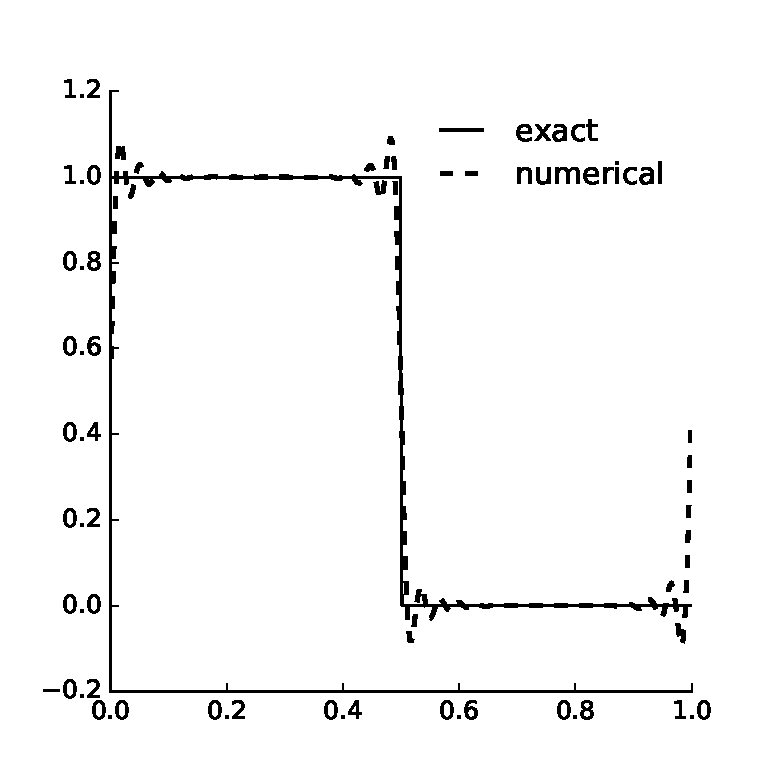
\includegraphics[width=\textwidth]{figures/context/unlimited}
      \caption{Unlimited solution}
    \end{subfigure}
    \hfill
    \begin{subfigure}{0.45\textwidth}
      \centering
      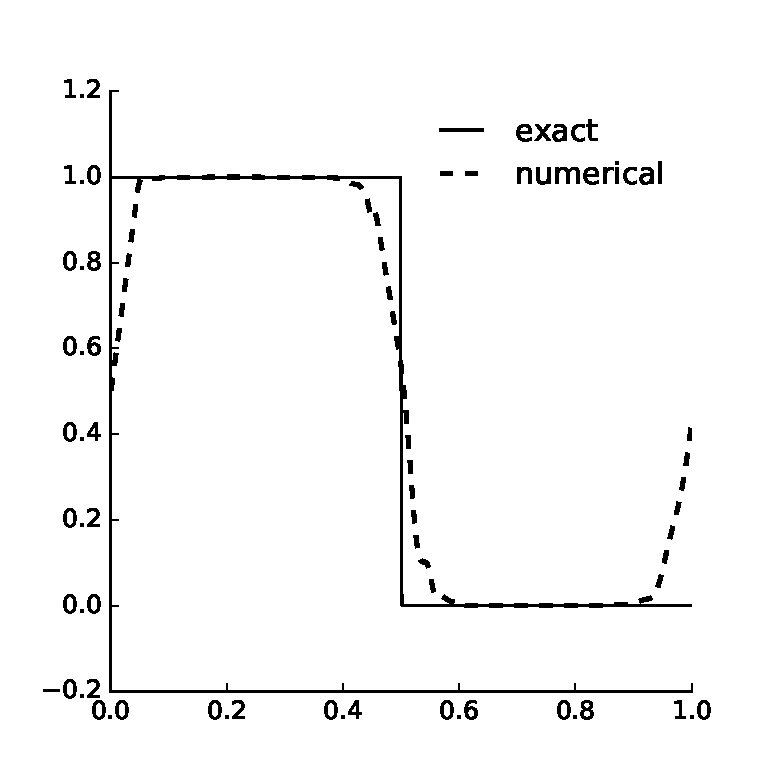
\includegraphics[width=\textwidth]{figures/context/minmod}
      \caption{With limiter}
    \end{subfigure}
    \caption{Linear advection of a square pulse}
  \end{figure}
\end{frame}

\begin{frame}
  \frametitle{Discontinuous Galerkin}
  \begin{itemize}
  \item Spatial domain $X = [a, b] \subset \mathbb{R}$
  \item Hyperbolic PDE $u_{t} + f(u)_{x} = 0$
  \item True solution $u(x, t) : X \times \mathbb{R}_{\ge 0} \rightarrow \mathbb{R}$
  \item Domain discretization into $n$ cells $[x_{i}, x_{i + 1}]$
  \item Time discretization $t_{0} < t_{1} < \dots$
  \item Piecewise continuous DG solution $U$ for every point in time $t_{i}$
  \end{itemize}
\end{frame}

\begin{frame}
  \frametitle{The structure of $U$}
  \begin{equation*}
    U = \bigoplus_{i = 0}^{n - 1} U_{i} \circ \xi_{i}
  \end{equation*}
  \begin{itemize}
  \item Direct sum of polynomials on individual cells
  \item $U_{i}$ is the solution on cell $i$
  \item $\xi_{i}$ maps cell coordinates to the reference interval $[-1, 1]$
  \end{itemize}
\end{frame}

\begin{frame}
  \frametitle{The $U_{i}$ in the Legendre basis}
  \begin{equation*}
    U_{i} = \sum_{j = 0}^{p} c_{i}^{j} P_{j}
  \end{equation*}

  \vspace{2em}

  \begin{description}
  \item[$P_{j}$] $j$-th Legendre polynomial
  \item[$c_{i}^{j}$] Coefficients
  \end{description}
\end{frame}

\begin{frame}
  \frametitle{Mapping to the reference interval}
  \begin{minipage}{0.7\textwidth}
    \begin{align*}
      \xi_{i}(x) & = 2 \frac{x - x_{i}}{x_{i + 1} - x_{i}} - 1\\
      \xi_{i}'(x) & = \frac{2}{x_{i + 1} - x_{i}} = \frac{2}{\Delta x_{i}}\\
      (\xi_{i}^{-1})'(x) & = \frac{\Delta x_{i}}{2}
    \end{align*}

    % \vspace{2em}

    % {\bf Note}: The center is mapped to $0$.
    % Thus $c_{i}^{0}$ models the
  \end{minipage}%
  \begin{minipage}{0.3\textwidth}
    \vspace{1em}
    \begin{figure}
      \centering
      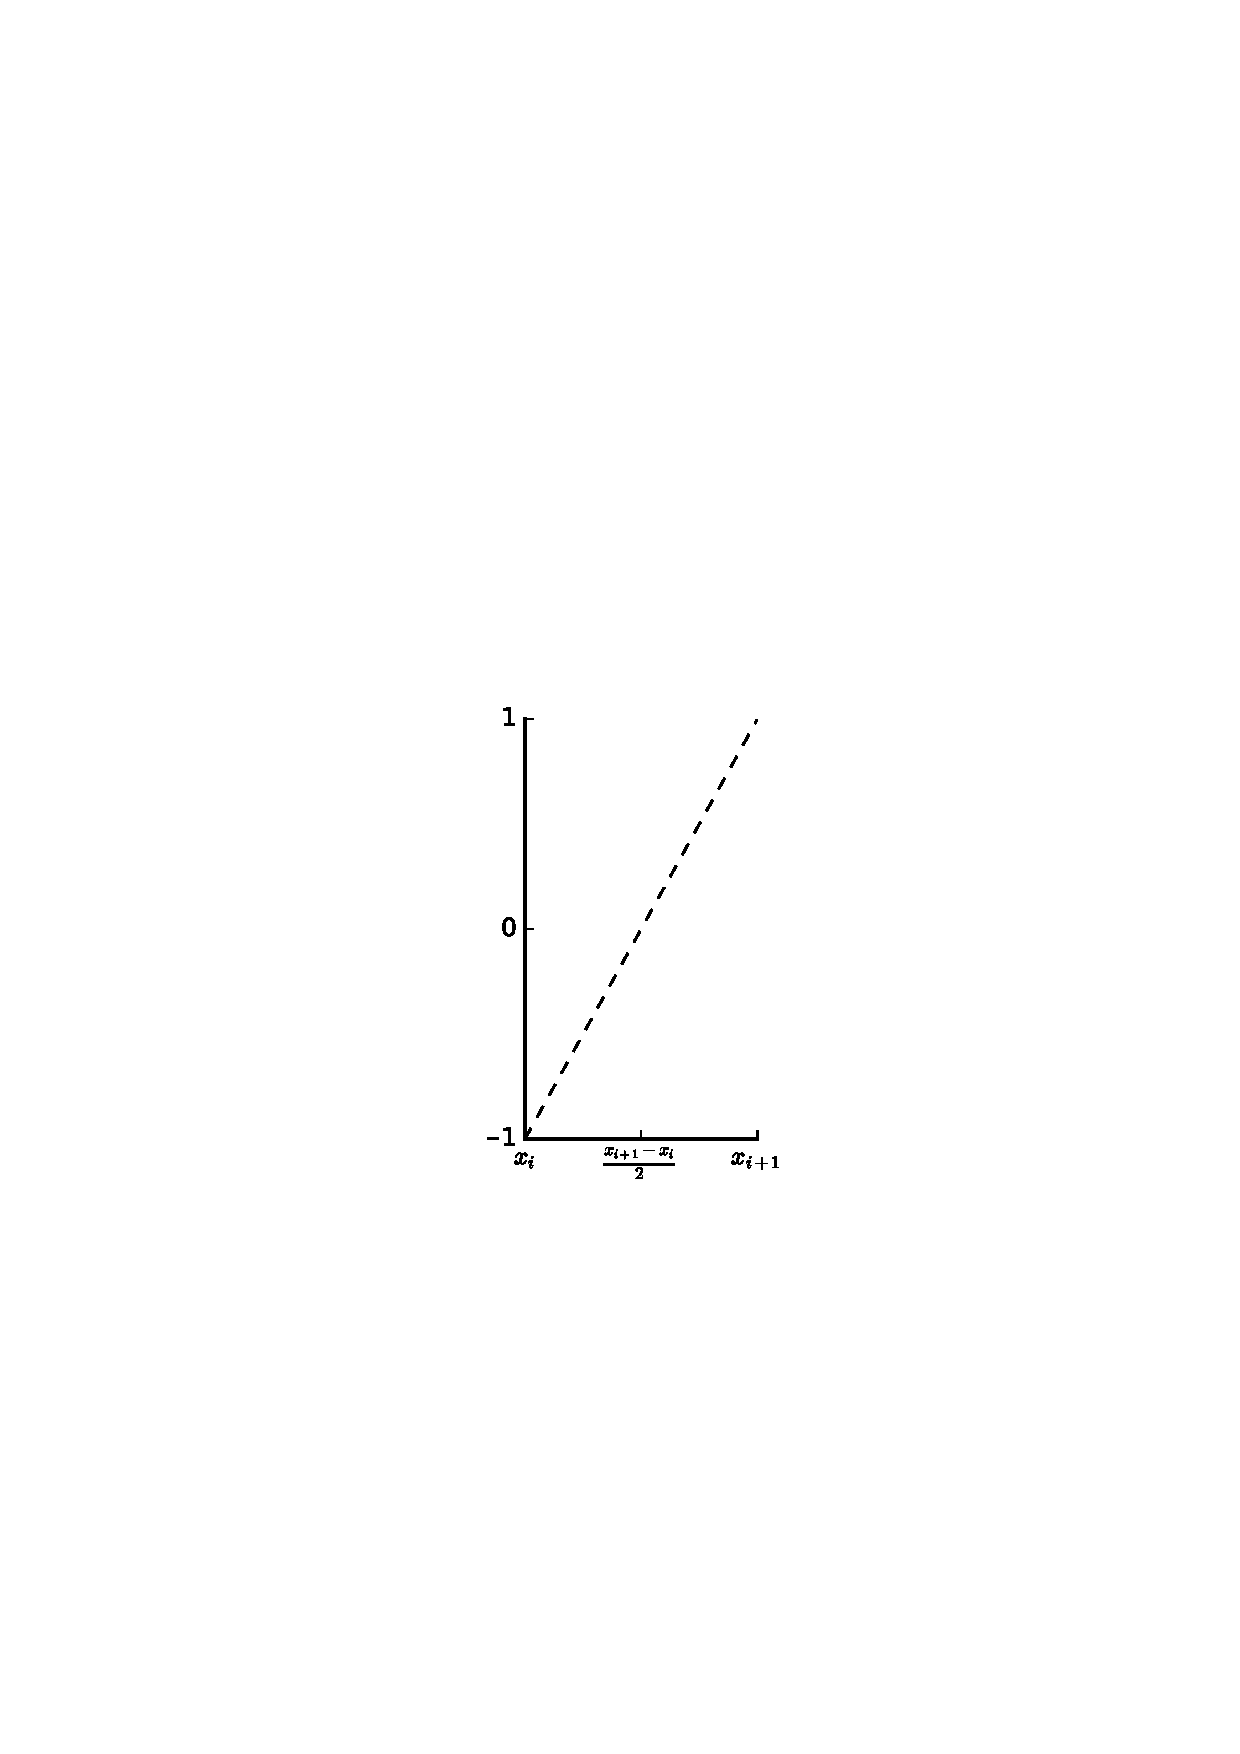
\includegraphics[width=\textwidth]{figures/dg/xi}
    \end{figure}
  \end{minipage}
\end{frame}

\begin{frame}
  \frametitle{The first-order special case}
  \begin{figure}[h]
    \centering
    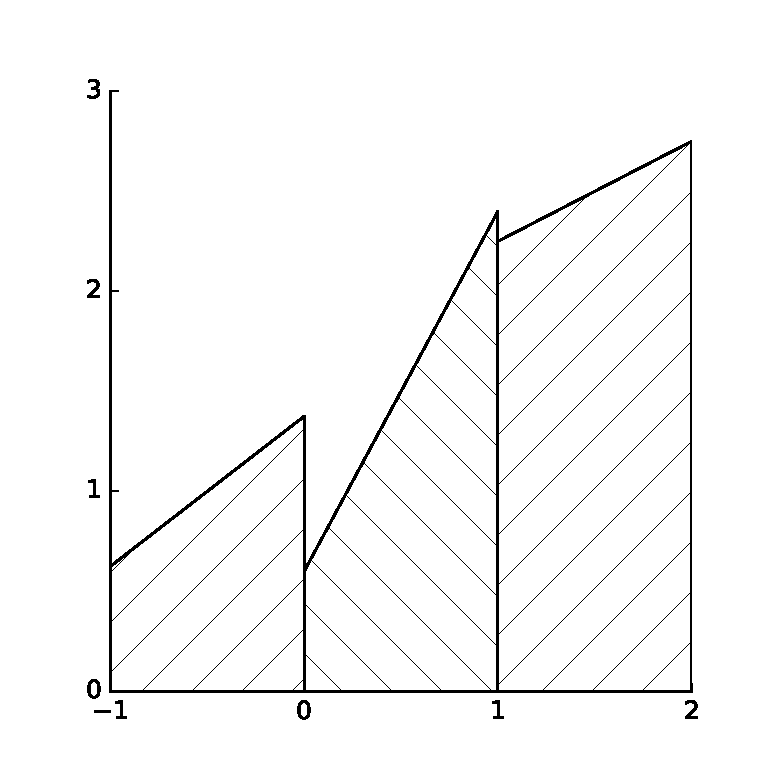
\includegraphics[width=0.5\textwidth]{figures/minmod/setup}
  \end{figure}
  \begin{equation*}
    U_{i}(x) = c_{i}^{1}x + c_{i}^{0}
  \end{equation*}
\end{frame}

\begin{frame}
  \frametitle{The minmod limiter}
  \begin{equation*}
    \tilde{c}_{i}^{1} = \minmod\left( c_{i}^{1}, \frac{c_{i + 1}^{0} - c_{i}^{0}}{\Delta x}, \frac{c_{i}^{0} - c_{i - 1}^{0}}{\Delta x} \right)
  \end{equation*}
  \vspace{1.5em}
  \begin{equation*}
    \minmod(a, b, c) = \begin{cases}
      \displaystyle\argmin_{x \in \{ a, b, c \}} |x| & \text{if} \sgn(a) = \sgn(b) = \sgn(c)\\
      0 & \text{otherwise}
    \end{cases}
  \end{equation*}
\end{frame}

\begin{frame}
  \frametitle{Scenarios of activity}
  \begin{figure}[h]
    \centering
    \begin{subfigure}{0.3\textwidth}
      \centering
      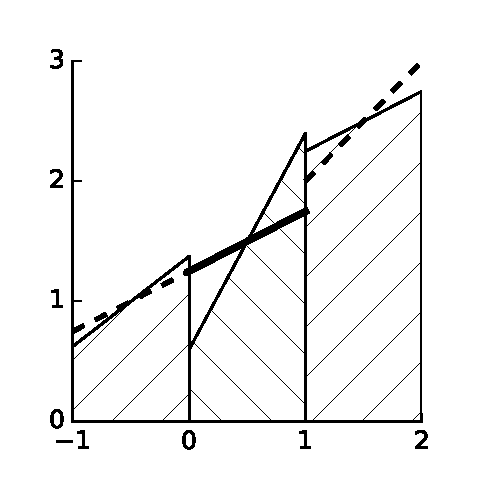
\includegraphics[width=\textwidth]{figures/minmod/steepness}
      \caption{Steepness}
    \end{subfigure}
    \hfill
    \begin{subfigure}{0.3\textwidth}
      \centering
      \includegraphics[width=\textwidth]{figures/minmod/extremum}
      \caption{Extremum}
    \end{subfigure}
    \hfill
    \begin{subfigure}{0.3\textwidth}
      \centering
      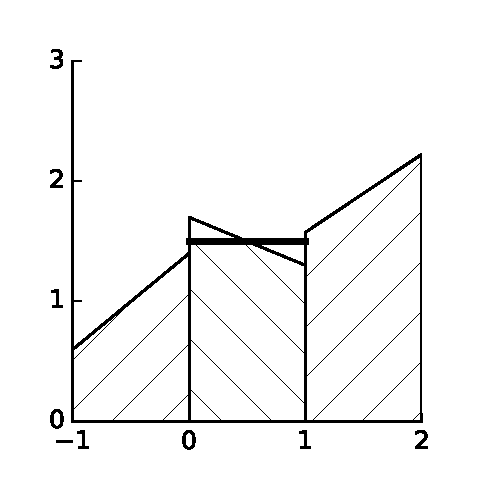
\includegraphics[width=\textwidth]{figures/minmod/disagreement}
      \caption{Disagreement}
    \end{subfigure}
  \end{figure}

  \begin{center}
    But why does this prevent oscillations?
  \end{center}
\end{frame}

\begin{frame}
  \frametitle{Total Variation}
  \begin{equation*}
    TV(f) = \sup_{\xi_{0}, \xi_{1}, \dots, \xi_{N}} \sum_{n = 1}^{N} \big| f(\xi_{n}) - f(\xi_{n - 1}) \big|
  \end{equation*}
  \begin{figure}[h]
    \centering
    \begin{subfigure}{0.3\textwidth}
      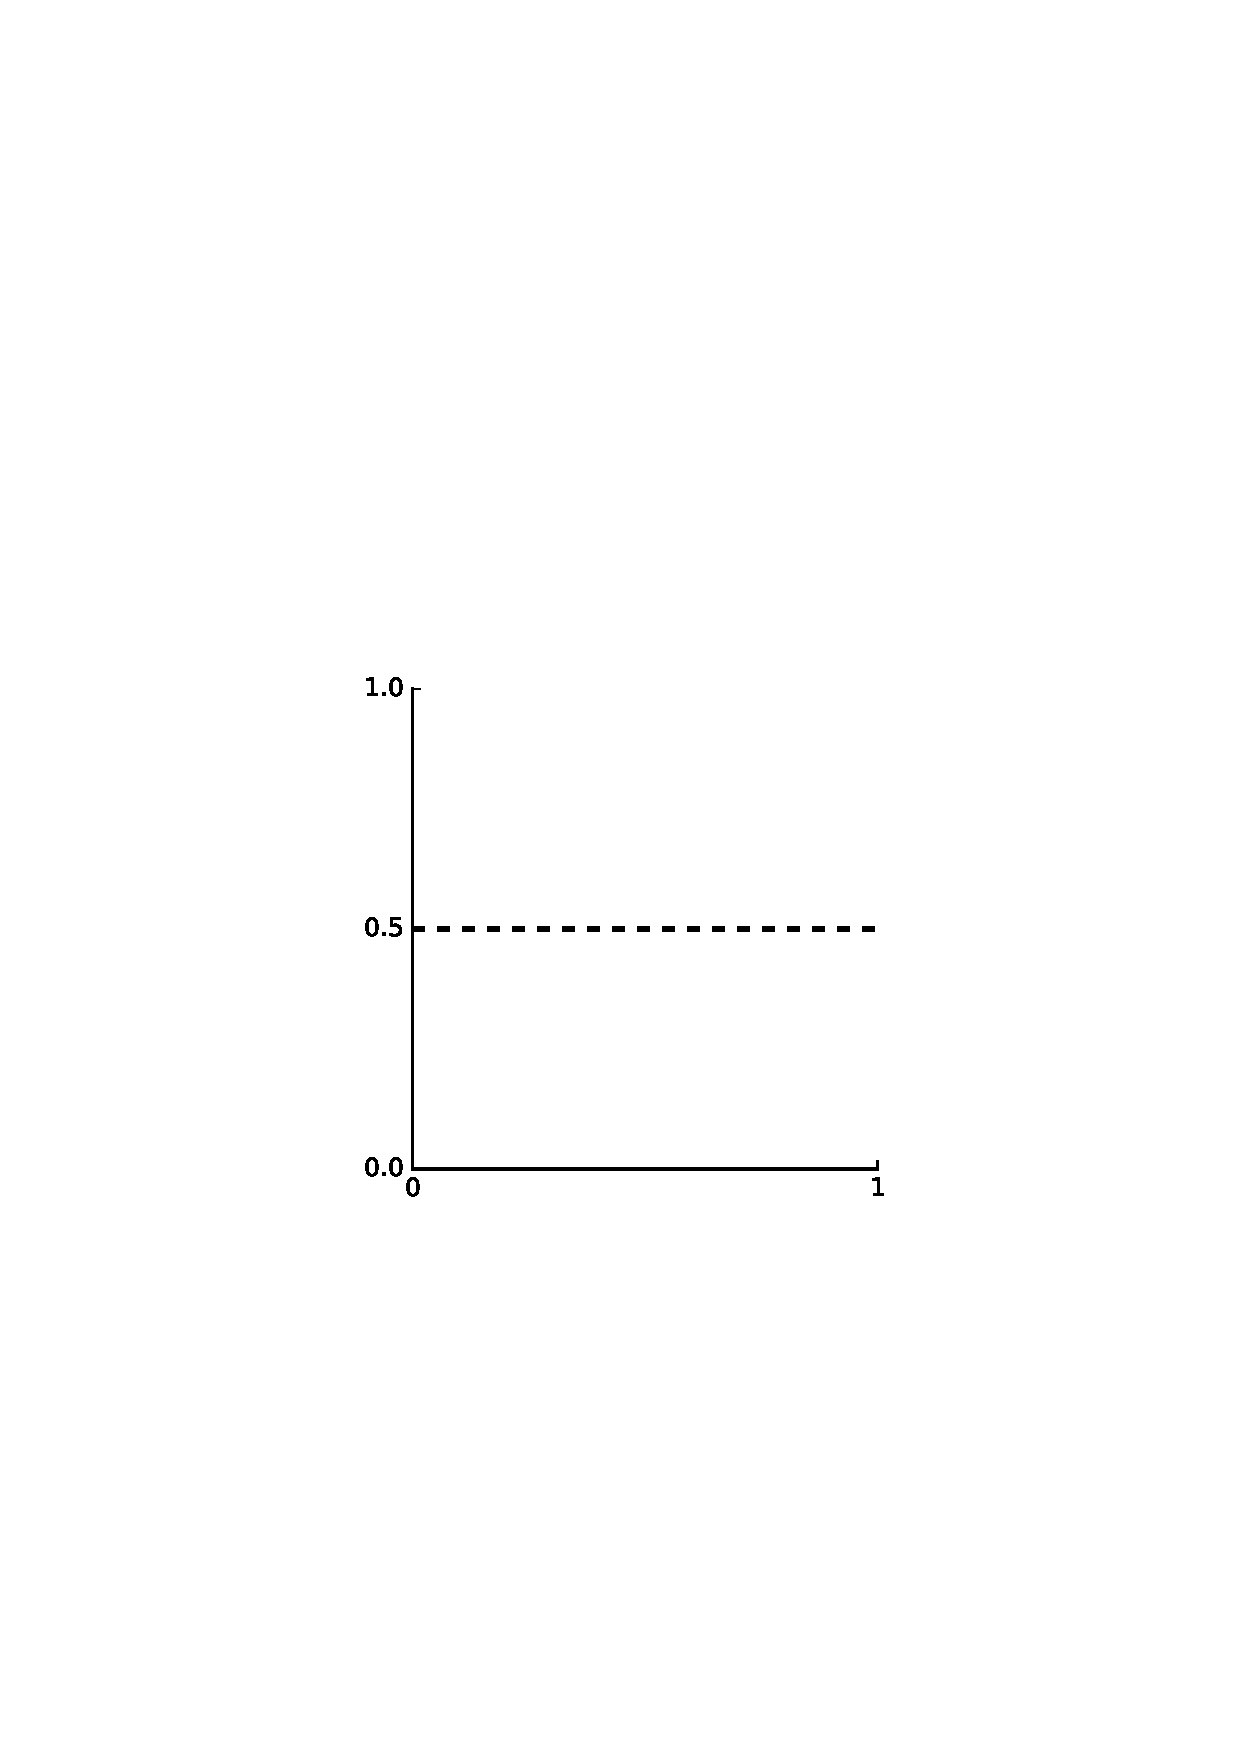
\includegraphics[width=\textwidth]{figures/tv/constant}
      \caption{$TV = 0$}
    \end{subfigure}
    \begin{subfigure}{0.3\textwidth}
      \includegraphics[width=\textwidth]{figures/tv/linear}
      \caption{$TV = 1$}
    \end{subfigure}
    \begin{subfigure}{0.3\textwidth}
      \includegraphics[width=\textwidth]{figures/tv/higher}
      \caption{$TV = 2$}
    \end{subfigure}
  \end{figure}
\end{frame}

\begin{frame}
  \frametitle{Why is total variation relevant?}
  \begin{itemize}
  \item \emph{monotone} methods never produce oscillations
  \item The true solution has constant total variation
  \item monotone schemes are \emph{total variation non-increasing} (TVNI/TVD)
  \item monotone schemes are at most first-order accurate
  \item Numerical methods should mimic this
  \item minmod is TVD
  \end{itemize}
\end{frame}

\begin{frame}
  \frametitle{How minmod minimizes TV}
  Each effect minimizes the TV
  \begin{figure}[h]
    \centering
    \begin{subfigure}{0.3\textwidth}
      \centering
      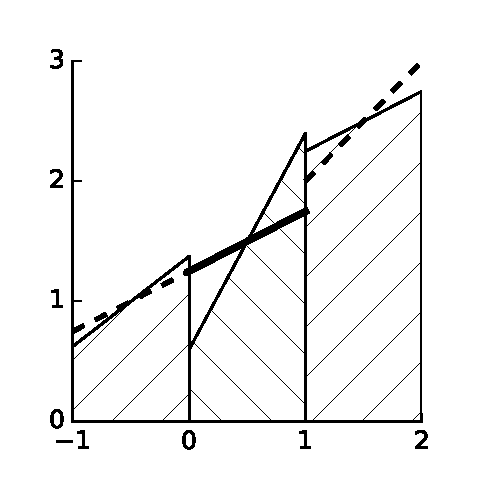
\includegraphics[width=\textwidth]{figures/minmod/steepness}
      \caption{Steepness}
    \end{subfigure}
    \hfill
    \begin{subfigure}{0.3\textwidth}
      \centering
      \includegraphics[width=\textwidth]{figures/minmod/extremum}
      \caption{Extremum}
    \end{subfigure}
    \hfill
    \begin{subfigure}{0.3\textwidth}
      \centering
      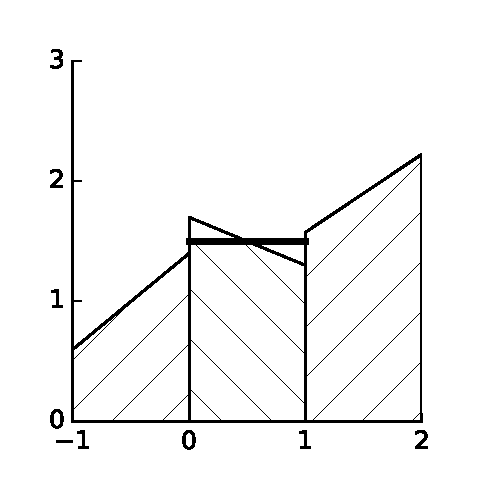
\includegraphics[width=\textwidth]{figures/minmod/disagreement}
      \caption{Disagreement}
    \end{subfigure}
  \end{figure}
\end{frame}

\begin{frame}
  \frametitle{Why minmod is still not perfect}
  \begin{itemize}
  \item Not directly applicable to higher-order models
  \item Order reduction near extrema
  \item Too diffusive
  \end{itemize}

  \vspace{2em}

  What can we do about this?
  \begin{itemize}
  \item Consider $U_{i} = \sum_{j = 0}^{p} c_{i}^{j} P_{j}$ of degree $p$ instead of $1$
  \item Extend minmod
  \item Relax limiter by limiting higher derivatives first
  \end{itemize}
\end{frame}

\begin{frame}
  \frametitle{The moment limiter}
  \begin{enumerate}
  \item Initialize $k := p$
  \item Compute $\tilde{c}_{i}^{k}$
  \item If $\tilde{c}_{i}^{k} \ne c_{i}^{k}$, reduce $k$ by $1$ and go back to step 1
  \item Finally replace all $c_{i}^{k}$ by $\tilde{c}_{i}^{k}$
  \end{enumerate}

  \vspace{1.5em}

  \begin{equation*}
    \tilde{c}_{i}^{k} = \minmod\left( c_{i}^{k}, c_{i + 1}^{k - 1} - c_{i}^{k - 1}, c_{i}^{k - 1} - c_{i - 1}^{k - 1} \right)
  \end{equation*}
\end{frame}

\begin{frame}
  \frametitle{Coefficient-derivative quasi-equivalence}
  Take a Taylor expansion of $u(\xi_{i}^{-1}(x))$ around some point $a$
  \begin{equation*}
    \sum_{n = 0}^{\infty} \frac{(x - a)^{n}}{n!} \partial_{x}^{n} u(\xi_{i}^{-1}(a)) = \sum_{n = 0}^{\infty} \frac{(x - a)^{n}}{n!} \frac{\Delta x_{i}}{2} \partial_{\xi_{i}^{-1}}^{n} u(\xi_{i}^{-1}(a))
  \end{equation*}
  and equate the coefficients with
  \begin{equation*}
    U_{i}(x - a) = \sum_{j = 0}^{p} c_{i}^{j} P_{j}(x - a)
  \end{equation*}
  to receive
  \begin{equation*}
    c_{i}^{j} \approx C \Delta x_{i} \partial_{x}^{j} u(\xi_{i}^{-1}(a))
  \end{equation*}
\end{frame}

\begin{frame}
  \frametitle{Computing the $k$-th derivative of $U_{i}$ -- I}
  \begin{equation*}
    \text{Leading coefficient of $P_{j}$ is $\frac{(2j)!}{2^{j}j!j!}$} \Rightarrow \partial_{x}^{j} P_{j}(x) = \frac{(2j)!}{2^{j} j!j!} \cdot j! = \frac{(2j)!}{2^{j} j!}
  \end{equation*}
  \begin{flalign*}
    & \partial_{x}^{k} (U_{i} \circ \xi_{i})(x) = \sum_{j = 0}^{p} c_{i}^{j} \partial_{x}^{k} P_{j}(\xi_{i}(x))&\\
    \intertext{The first $k - 1$ terms vanish}
    =~& \sum_{j = k}^{p} c_{i}^{j} \partial_{x}^{k} P_{j}(\xi_{i}(x))&\\
    \intertext{Apply the chain rule $k$ times}
    =~& \sum_{j = k}^{p} c_{i}^{j} \left( \frac{2}{\Delta x_{i}} \right)^{k} \partial_{\xi_{i}}^{k} P_{j}(\xi_{i}(x))&
  \end{flalign*}
\end{frame}

\begin{frame}
  \frametitle{Computing the $k$-th derivative of $U_{i}$ -- II}
  \begin{flalign*}
    \intertext{Separate the first summand}
    =~& c_{i}^{k} \left( \frac{2}{\Delta x_{i}} \right)^{k} \partial_{\xi_{i}}^{k} P_{k}(\xi_{i}(x)) + \sum_{j = k + 1}^{p} c_{i}^{j} \left( \frac{2}{\Delta x_{i}} \right)^{k} \partial_{\xi_{i}}^{k} P_{j}(\xi_{i}(x))&\\
    \intertext{Plug in the $k$-th derivative of $P_{k}$}
    =~& c_{i}^{k} \left( \frac{2}{\Delta x_{i}} \right)^{k} \frac{(2k)!}{2^{k} k!} + \sum_{j = k + 1}^{p} c_{i}^{j} \left( \frac{2}{\Delta x_{i}} \right)^{k} \partial_{\xi_{i}}^{k} P_{j}(\xi_{i}(x))&\\
    \intertext{Simplify}
    =~& c_{i}^{k} \left( \frac{2}{\Delta x_{i}} \right)^{k} \left( 2k - 1 \right)!! + \sum_{j = k + 1}^{p} c_{i}^{j} \left( \frac{2}{\Delta x_{i}} \right)^{k} \partial_{\xi_{i}}^{k} P_{j}(\xi_{i}(x))&
  \end{flalign*}
\end{frame}

\begin{frame}
  \frametitle{First-order approximations to the $k$-th derivative -- I}
  Plug in $k - 1$ for $k$ to get the $k - 1$-th derivative
  \begin{align*}
    \partial_{x}^{k - 1} U_{i} \circ \xi_{i}(x) & = \left( \frac{2}{\Delta x_{i}} \right)^{k - 1} \left( 2k - 3 \right)!!~c_{i}^{k - 1}\\
    & \quad + \sum_{j = k}^{p} c_{i}^{j} \left( \frac{2}{\Delta x_{i}} \right)^{k - 1} \partial_{\xi_{i}}^{k - 1} P_{j}(\xi_{i}(x))
  \end{align*}
\end{frame}

\begin{frame}
  \frametitle{First-order approximations to the $k$-th derivative -- II}
  Compute the forward and backward difference quotients
  \begin{align*}
    & \frac{\partial_{x}^{k - 1} (U_{i + 1} \circ \xi_{i + 1})(x) - \partial_{x}^{k - 1} (U_{i} \circ \xi_{i})(x)}{\Delta x_{i}}\\
    =~& \left( \frac{2}{\Delta x_{i}} \right)^{k} \frac{(2k - 3)!!}{2} (c_{i + 1}^{k - 1} - c_{i}^{k - 1})\\
    & + \frac{1}{2} \left( \frac{2}{\Delta x_{i}} \right)^{k} \sum_{j = k}^{p} (c_{i + 1}^{j} - c_{i}^{j}) \partial_{\xi_{i}}^{k - 1} P_{j}(\xi_{i}(x))
  \end{align*}
  \tiny{backward difference quotient omitted because it is basically the same}
\end{frame}

\begin{frame}
  \frametitle{Derivation of the moment limiter -- I}
  Equate the first summands of the $k$-th derivative and its first-order approximations
  \begin{equation*}
    \left( \frac{2}{\Delta x_{i}} \right)^{k} \left( 2k - 1 \right)!!~c_{i}^{k} = \left( \frac{2}{\Delta x_{i}} \right)^{k} \frac{(2k - 3)!!}{2} (c_{i + 1}^{k - 1} - c_{i}^{k - 1})
  \end{equation*}
  \begin{equation*}
    \left( \frac{2}{\Delta x_{i}} \right)^{k} \left( 2k - 1 \right)!!~c_{i}^{k} = \left( \frac{2}{\Delta x_{i}} \right)^{k} \frac{(2k - 3)!!}{2} (c_{i}^{k - 1} - c_{i - 1}^{k - 1})
  \end{equation*}
  to get the approximations
  \begin{equation*}
    c_{i}^{k} \approx \frac{c_{i + 1}^{k - 1} - c_{i}^{k - 1}}{2(2k - 1)} \quad \text{and} \quad c_{i}^{k} \approx \frac{c_{i}^{k - 1} - c_{i - 1}^{k - 1}}{2(2k - 1)}
  \end{equation*}
\end{frame}

\begin{frame}
  \frametitle{Derivation of the moment limiter -- II}
  Using these in the same fashion as minmod we get
  \begin{equation*}
    \tilde{c}_{i}^{k} = \minmod\left( c_{i}^{k}, \frac{c_{i + 1}^{k - 1} - c_{i}^{k - 1}}{2(2k - 1)}, \frac{c_{i}^{k - 1} - c_{i - 1}^{k - 1}}{2(2k - 1)} \right)
  \end{equation*}

  However, this is too diffusive so it was generalized to
  \begin{equation*}
    \tilde{c}_{i}^{k} = \minmod\left( c_{i}^{k}, \alpha_{i} \left( c_{i + 1}^{k - 1} - c_{i}^{k - 1} \right), \alpha_{i} \left( c_{i}^{k - 1} - c_{i - 1}^{k - 1} \right) \right)
  \end{equation*}
  for $\frac{1}{2(2k - 1)} \le \alpha_{i} \le 1$
\end{frame}

\begin{frame}
  \frametitle{Numerical Results}
  \begin{figure}[h]
    \centering
    \begin{subfigure}{0.35\textwidth}
      \centering
      \includegraphics[width=\textwidth]{figures/results/moment-p-1}
      \caption{$p = 1$}
    \end{subfigure}
    \hspace{2em}
    \begin{subfigure}{0.35\textwidth}
      \centering
      \includegraphics[width=\textwidth]{figures/results/moment-p-4}
      \caption{$p = 4$}
    \end{subfigure}
    \caption{Advection results and limiter activity\footnote{Krivodonova, ``Limiters for high-order discontinuous galerkin methods''}}
  \end{figure}
\end{frame}

\begin{frame}
  \frametitle{Open Questions}
  \begin{itemize}
  \item How is the exact relation between coefficients and derivatives?
  \item Can you prove that the moment limiter is TVB?
  \item Can it be made TVD?
  \item Does it work for other basis functions?
  \end{itemize}
\end{frame}

\begin{frame}[standout]
  \vfill
  \Huge{Questions?}
  \vfill
\end{frame}

\appendix

\begin{frame}[allowframebreaks]
  \frametitle{References}
  \nocite{Krivodonova}
  \nocite{Biswas1994}
  \nocite{Harten1983}
  \nocite{VanLeer1979}
  \bibliographystyle{amsalpha}
  \bibliography{../case-study/references.bib}
\end{frame}

\end{document}
